\documentclass{report}
\usepackage[a4paper, total={7.5in, 10in}]{geometry}
\usepackage[fleqn]{amsmath}
\usepackage{amssymb}
\usepackage{amsthm}
\usepackage{enumitem}
\usepackage[]{mdframed}
\usepackage{multicol}
\usepackage{thmtools}
\usepackage{graphicx}
\usepackage{tikz}
\usepackage{tipa}

\usepackage{ifxetex}

\ifxetex
    \usepackage{substitutefont}
    \substitutefont{T3}{\rmdefault}{cmr}
\fi

\usepackage{fontspec}
\setmainfont[Mapping=tex-text]{Times New Roman}

\title{Praktis 2\\Differentiation}
\author{Melvin Chia}

\newcommand{\sol}[1]{

    \noindent \textbf{Sol.}
}
\newcommand{\prooff}[1]{

    \noindent \textbf{Proof.}
}

\newcommand{\arc}[1]{{%
            \setbox9=\hbox{#1}%
            \ooalign{\resizebox{\wd9}{\height}{\texttoptiebar{\phantom{A}}}\cr#1}}}

\def\eos{\quad\hbox{\rlap{\hbox{\vrule depth 1.5pt height 2.6mm width 0.2mm \hskip 1mm \vrule height 2.6mm width 0.2mm}}{\vbox{\hrule height 0.2mm width 1.4mm \vskip 2.8mm \hrule depth 1.5pt height -0.35mm width 1.2mm}}}}

\counterwithout{equation}{chapter}
\setlength{\columnseprule}{1pt}
\setlength{\columnsep}{24pt}
\hfuzz=100pt
\setcounter{chapter}{2}

\mdfdefinestyle{MyFrame}{%
    linecolor=black,
    linewidth=1pt,
    roundcorner=20pt,
    innertopmargin=12pt, innerbottommargin=12pt, innerrightmargin=12pt,
    innerleftmargin=12pt, leftmargin = 4pt, rightmargin = 4pt
    %backgroundcolor=gray!50!white}
}

\begin{document}
\maketitle

\begin{multicols*}{2}
    \section{Limit and its Relation to Differentiation}
    \begin{enumerate}
        \item Find the value of each of the following.
              \begin{enumerate}
                  \item $\lim\limits_{x\to1}(x-1)$
                        \sol{}
                        \begin{flalign*}
                            \lim\limits_{x\to1}(x-1) & = 1 - 1  \\
                                                     & = 0 \eos
                        \end{flalign*}

                  \item $\lim\limits_{x\to1}{\dfrac{x^{2}-2}{x}}$
                        \sol{}
                        \begin{flalign*}
                            \lim\limits_{x\to1}{\dfrac{x^{2}-2}{x}} & = \dfrac{1^{2}-2}{1} \\
                                                                    & = \dfrac{-1}{1}      \\
                                                                    & = -1 \eos
                        \end{flalign*}

                  \item $\lim\limits_{x\to0}{\dfrac{2x-5}{x+3}}$
                        \sol{}
                        \begin{flalign*}
                            \lim\limits_{x\to0}{\dfrac{2x-5}{x+3}} & = \dfrac{2(0)-5}{0+3} \\
                                                                   & = \dfrac{-5}{3}       \\
                                                                   & = -\dfrac{5}{3} \eos
                        \end{flalign*}

                  \item $\lim\limits_{x\rightarrow a}(x-a)$
                        \sol{}
                        \begin{flalign*}
                            \lim\limits_{x\rightarrow a}(x-a) & = a - a  \\
                                                              & = 0 \eos
                        \end{flalign*}
              \end{enumerate}
        \item Calculate the value for each of the following.
              \begin{enumerate}
                  \item $\lim\limits_{x\to0}{\dfrac{2x^{2}-5x}{x}}$
                        \sol{}
                        \begin{flalign*}
                            \lim\limits_{x\to0}{\dfrac{2x^{2}-5x}{x}} & = \lim\limits_{x\to0}{\dfrac{x(2x-5)}{x}} \\
                                                                      & = \lim\limits_{x\to0}{(2x-5)}             \\
                                                                      & = 2(0) - 5                                \\
                                                                      & = -5 \eos
                        \end{flalign*}

                  \item $\lim\limits_{x\to2}{\dfrac{x^{2}-4}{x-2}}$
                        \sol{}
                        \begin{flalign*}
                            \lim\limits_{x\to2}{\dfrac{x^{2}-4}{x-2}} & = \lim\limits_{x\to2}{\dfrac{(x-2)(x+2)}{x-2}} \\
                                                                      & = \lim\limits_{x\to2}{(x+2)}                   \\
                                                                      & = 2 + 2                                        \\
                                                                      & = 4 \eos
                        \end{flalign*}

                  \item $\lim\limits_{x\to5}{\dfrac{x^{2}+4x-45}{x-5}}$
                        \sol{}
                        \begin{flalign*}
                            \lim\limits_{x\to5}{\dfrac{x^{2}+4x-45}{x-5}} & = \lim\limits_{x\to5}{\dfrac{(x-5)(x+9)}{x-5}} \\
                                                                          & = \lim\limits_{x\to5}{(x+9)}                   \\
                                                                          & = 5 + 9                                        \\
                                                                          & = 14 \eos
                        \end{flalign*}
                  \item $\lim\limits_{x\to1}{\dfrac{\log_{\mathrm{10}}x^{2}}{\log_{\mathrm{10}}x}}$
                        \sol{}
                        \begin{flalign*}
                            \lim\limits_{x\to1}{\dfrac{\log_{\mathrm{10}}x^{2}}{\log_{\mathrm{10}}x}} & = \lim\limits_{x\to1}{\dfrac{\log_{\mathrm{10}}x^{2}}{\log_{\mathrm{10}}x}} \\
                                                                                                      & = \lim\limits_{x\to1}{\dfrac{2\log_{\mathrm{10}}x}{\log_{\mathrm{10}}x}}    \\
                                                                                                      & = \lim\limits_{x\to1}{2}                                                    \\
                                                                                                      & = 2 \eos
                        \end{flalign*}
              \end{enumerate}
        \item Find the value for each of the following.
              \begin{enumerate}
                  \item $\lim\limits_{x\to9}{\dfrac{x-9}{\sqrt{x}-3}}$
                        \sol{}
                        \begin{flalign*}
                            \lim\limits_{x\to9}{\dfrac{x-9}{\sqrt{x}-3}} & = \lim\limits_{x\to9}{\dfrac{(x-9)'}{(\sqrt{x}-3)'}}   \\
                                                                         & = \lim\limits_{x\to9}{\dfrac{1}{\dfrac{1}{2\sqrt{x}}}} \\
                                                                         & = \lim\limits_{x\to9}{(2\sqrt{x})}                     \\
                                                                         & = 2\sqrt{9}                                            \\
                                                                         & = 2(3)                                                 \\
                                                                         & = 6 \eos
                        \end{flalign*}

                  \item $\lim\limits_{x\to-1}{\dfrac{x+1}{\sqrt{x+5}-2}}$
                        \sol{}
                        \begin{flalign*}
                            \lim\limits_{x\to-1}{\dfrac{x+1}{\sqrt{x+5}-2}} & = \lim\limits_{x\to-1}{\dfrac{(x+1)'}{(\sqrt{x+5}-2)'}}   \\
                                                                            & = \lim\limits_{x\to-1}{\dfrac{1}{\dfrac{1}{2\sqrt{x+5}}}} \\
                                                                            & = \lim\limits_{x\to-1}{(2\sqrt{x+5})}                     \\
                                                                            & = 2\sqrt{-1+5}                                            \\
                                                                            & = 2\sqrt{4}                                               \\
                                                                            & = 2(2)                                                    \\
                                                                            & = 4 \eos
                        \end{flalign*}

                  \item $\lim\limits_{x\to9}{\dfrac{\sqrt{x+7}-4}{x-9}}$
                        \sol{}
                        \begin{flalign*}
                            \lim\limits_{x\to9}{\dfrac{\sqrt{x+7}-4}{x-9}} & = \lim\limits_{x\to9}{\dfrac{(\sqrt{x+7}-4)'}{(x-9)'}} \\
                                                                           & = \lim\limits_{x\to9}{\dfrac{1}{2\sqrt{x+7}}}          \\
                                                                           & = \dfrac{1}{2\sqrt{9+7}}                               \\
                                                                           & = \dfrac{1}{8}                                         \\
                        \end{flalign*}
                  \item $\lim\limits_{x\to2}{\dfrac{\sqrt{6-x}-2}{3-{\sqrt{11-x}}}}$
                        \sol{}
                        \begin{flalign*}
                            \lim\limits_{x\to2}{\dfrac{\sqrt{6-x}-2}{3-{\sqrt{11-x}}}} & = \lim\limits_{x\to2}{\dfrac{(\sqrt{6-x}-2)'}{(3-{\sqrt{11-x}})'}}              \\
                                                                                       & = \lim\limits_{x\to2}{\dfrac{\dfrac{1}{2\sqrt{6-x}}}{\dfrac{1}{-2\sqrt{11-x}}}} \\
                                                                                       & = \lim\limits_{x\to2}{\dfrac{-2\sqrt{11-x}}{2\sqrt{6-x}}}                       \\
                                                                                       & = \lim\limits_{x\to2}{\dfrac{-\sqrt{11-x}}{\sqrt{6-x}}}                         \\
                                                                                       & = -\dfrac{\sqrt{11-2}}{\sqrt{6-2}}                                              \\
                                                                                       & = -\dfrac{3}{2} \eos
                        \end{flalign*}
              \end{enumerate}
        \item The following diagram shows part of a graph $y = f(x)$.
              \begin{center}
                  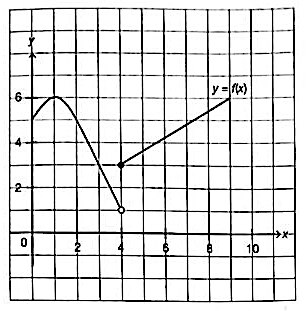
\includegraphics[width=0.4\textwidth]{./images/q4.jpeg}
              \end{center}
              Based on this graph, find
              \begin{enumerate}
                  \item $f(4)$
                        \sol{}
                        \begin{flalign*}
                            f(4) & = 3
                        \end{flalign*}

                  \item $\lim\limits_{x\to4}{f(x)}$ and explain your answer.
                        \sol{}
                        \begin{flalign*}
                            \lim_{x\to4^-}{f(x)} & \neq 4 \\
                            \lim_{x\to4^+}{f(x)} & = 4    \\
                        \end{flalign*}
                        Since the left limit and right limit are different, $f(4)$ does not exist.

                  \item $\lim\limits_{x\to1}{f(x)}$
                        \sol{}
                        \begin{flalign*}
                            \lim_{x\to1}{f(x)} & = 6 \\
                        \end{flalign*}
              \end{enumerate}

        \item Find $\dfrac{dy}{dx}$ by using the first principle.
              \begin{enumerate}
                  \item $y = 3x + 5$
                        \sol{}
                        \begin{flalign*}
                            y                          & = 3x + 5                                                              & (1) \\
                            y + \delta y               & = 3(x + \delta x) + 5                                                       \\
                            y + \delta y               & = 3x + 3\delta x + 5                                                  & (2) \\
                            (2) - (1):                 &                                                                             \\
                            \delta y                   & = 3\delta x                                                                 \\
                            \dfrac{\delta y}{\delta x} & = 3                                                                         \\
                            \therefore\ \dfrac{dy}{dx} & = \lim\limits_{\delta x\to0}{\left(\dfrac{\delta y}{\delta x}\right)}       \\
                                                       & = \lim\limits_{\delta x\to0}{3}                                             \\
                                                       & = 3 \eos
                        \end{flalign*}

                  \item $y = x^2 - 7$
                        \sol{}
                        \begin{flalign*}
                            y                          & = x^2 - 7                                                             & (1) \\
                            y + \delta y               & = (x + \delta x)^2 - 7                                                      \\
                            y + \delta y               & = x^2 + 2x\delta x + {(\delta x)}^2 - 7                               & (2) \\
                            (2) - (1):                 &                                                                             \\
                            \delta y                   & = 2x\delta x + {(\delta x)}^2                                               \\
                            \dfrac{\delta y}{\delta x} & = 2x + 2\delta x                                                            \\
                            \therefore\ \dfrac{dy}{dx} & = \lim\limits_{\delta x\to0}{\left(\dfrac{\delta y}{\delta x}\right)}       \\
                                                       & = \lim\limits_{\delta x\to0}{(2x + 2\delta x)}                              \\
                                                       & = 2x \eos
                        \end{flalign*}

                  \item $y = x^2 + 2x + 1$
                        \sol{}
                        \begin{flalign*}
                            y                          & = x^2 + 2x + 1                                                        & (1) \\
                            y + \delta y               & = (x + \delta x)^2 + 2(x + \delta x) + 1                                    \\
                            y + \delta y               & = x^2 + 2x\delta x + {(\delta x)}^2 + 2x + 2\delta x                        \\
                                                       & \ \ \ \ + 1                                                           & (2) \\
                            (2) - (1):                 &                                                                             \\
                            \delta y                   & = 2x\delta x + {(\delta x)}^2 + 2\delta x                                   \\
                            \dfrac{\delta y}{\delta x} & = 2x + \delta x + 2                                                         \\
                            \therefore\ \dfrac{dy}{dx} & = \lim\limits_{\delta x\to0}{\left(\dfrac{\delta y}{\delta x}\right)}       \\
                                                       & = \lim\limits_{\delta x\to0}{(2x + \delta x + 2)}                           \\
                                                       & = 2x + 2 \eos
                        \end{flalign*}

                  \item $y = -x^3 + 9$
                        \sol{}
                        \begin{flalign*}
                            y                          & = -x^3 + 9                                                                     & (1) \\
                            y + \delta y               & = -(x + \delta x)^3 + 9                                                              \\
                            y + \delta y               & = -x^3 - 3x^2\delta x - 3x{(\delta x)}^2 - \delta x^3                                \\
                                                       & \ \ \ \ + 9                                                                    & (2) \\
                            (2) - (1):                 &                                                                                      \\
                            \delta y                   & = -3x^2\delta x - 3x{(\delta x)}^2 - \delta x^3                                      \\
                            \dfrac{\delta y}{\delta x} & = -3x^2 - 3x\delta x - {(\delta x)}^2                                                \\
                            \therefore\ \dfrac{dy}{dx} & = \lim\limits_{\delta x\to0}{\left(\dfrac{\delta y}{\delta x}\right)}                \\
                                                       & = \lim\limits_{\delta x\to0}{\left[-3x^2 - 3x\delta x - {(\delta x)}^2\right]}       \\
                                                       & = -3x^2 \eos
                        \end{flalign*}

                  \item $y = 2 - \dfrac{3}{x}$
                        \sol{}
                        \begin{flalign*}
                            y                          & = 2 - 3x^{-1}                                                         & (1) \\
                            y + \delta y               & = 2 - 3{(x + \delta x)}^{-1}                                          & (2) \\
                            (2) - (1):                 &                                                                             \\
                            \delta y                   & = -3{(x + \delta x)}^{-1} + 3x^{-1}                                         \\
                                                       & = -\frac{3}{x + \delta x} + \frac{3}{x}                                     \\
                                                       & = \frac{-3x + 3x + 3\delta x}{x(x + \delta x)}                              \\
                                                       & = \frac{3\delta x}{x^2 + x\delta x}                                         \\
                            \dfrac{\delta y}{\delta x} & = \frac{3}{x^2 + x\delta x}                                                 \\
                            \therefore\ \dfrac{dy}{dx} & = \lim\limits_{\delta x\to0}{\left(\dfrac{\delta y}{\delta x}\right)}       \\
                                                       & = \lim\limits_{\delta x\to0}{\left(\frac{3}{x^2 + x\delta x}\right)}        \\
                                                       & = \frac{3}{x^2} \eos
                        \end{flalign*}
              \end{enumerate}

        \item Given a curve $y = x^2 - ax + b$
              \begin{enumerate}
                  \item By using the first principle, find the gradient function to the curve. \sol{}
                        \begin{flalign*}
                            y                          & = x^2 - ax + b                                                        & (1) \\
                            y + \delta y               & = (x + \delta x)^2 - a(x + \delta x) + b                                    \\
                            y + \delta y               & = x^2 + 2x\delta x + {(\delta x)}^2 - ax - a\delta x                        \\
                                                       & \ \ \ \ + b                                                           & (2) \\
                            (2) - (1):                 &                                                                             \\
                            \delta y                   & = 2x\delta x + {(\delta x)}^2 - a\delta x                                   \\
                            \dfrac{\delta y}{\delta x} & = 2x + \delta x - a                                                         \\
                            \therefore\ \dfrac{dy}{dx} & = \lim\limits_{\delta x\to0}{\left(\dfrac{\delta y}{\delta x}\right)}       \\
                                                       & = \lim\limits_{\delta x\to0}{(2x + \delta x - a)}                           \\
                                                       & = 2x - a \eos
                        \end{flalign*}

                  \item Given that the value of gradient of the curve at $(2, -3)$ is $2$, find the
                        value of $a$ and $b$. \sol{}
                        \begin{flalign*}
                            \dfrac{dy}{dx} & = 2x - a             \\
                            2              & = 2(2) - a           \\
                            \therefore\ a  & = 2 \eos             \\
                            \\
                            y              & = x^2 - 2x + b       \\
                            -3             & = {(2)}^2 - 2(2) + b \\
                            -3             & = 4 - 4 + b          \\
                            \therefore\ b  & = -3 \eos
                        \end{flalign*}
              \end{enumerate}
    \end{enumerate}

    \section{The First Derivative}

    \begin{enumerate}
        \setcounter{enumi}{6}
        \item Find the first derivative for each of the following functions.
              \begin{enumerate}
                  \item $y = 6x^2$
                        \sol{}
                        \begin{flalign*}
                            \dfrac{dy}{dx} & = 12x \eos
                        \end{flalign*}

                  \item $y = -x^4$
                        \sol{}
                        \begin{flalign*}
                            \dfrac{dy}{dx} & = -4x^3 \eos
                        \end{flalign*}

                  \item $y = \sqrt[3]{x^4}$
                        \sol{}
                        \begin{flalign*}
                            y              & = x^{\frac{4}{3}}                \\
                            \dfrac{dy}{dx} & = \frac{4}{3}x^{\frac{4}{3} - 1} \\
                                           & = \frac{4}{3}\sqrt[3]{x} \eos
                        \end{flalign*}

                  \item $y = -\frac{2}{x^2}$
                        \sol{}
                        \begin{flalign*}
                            y              & = -2x^{-2}                \\
                            \dfrac{dy}{dx} & = -2\left(-2x^{-3}\right) \\
                                           & = 4x^{-3}                 \\
                                           & = \frac{4}{x^3} \eos
                        \end{flalign*}
              \end{enumerate}

        \item Find each of the following.
              \begin{enumerate}
                  \item ${\dfrac{d}{d x}}\Big(2x^{2}+3x-9{\Big)}$
                        \sol{}
                        \begin{flalign*}
                            \dfrac{d}{d x}\Big(2x^{2}+3x-9{\Big)} & = 4x + 3 \eos
                        \end{flalign*}
                  \item ${\dfrac{d}{d x}}\left(x^{2}+{\dfrac{2}{x}}\right)$
                        \sol{}
                        \begin{flalign*}
                            \dfrac{d}{d x}\left(x^{2}+{\dfrac{2}{x}}\right) & = \dfrac{d}{dx}\left(x^2 + 2x^{-1}\right) \\
                                                                            & = 2x -2x^{-2}                             \\
                                                                            & = 2x - \dfrac{2}{x^2}\eos
                        \end{flalign*}
                  \item ${\dfrac{d}{d x}}\left(5x^{3}+2x^{2}+4x-7-{\dfrac{1}{x}}+{\dfrac{3}{x^{2}}}\right)$
                        \sol{}
                        \begin{flalign*}
                             & \dfrac{d}{d x}\left(5x^{3}+2x^{2}+4x-7-{\dfrac{1}{x}}+{\dfrac{3}{x^{2}}}\right) \\
                             & = \dfrac{d}{d x}\left(5x^{3}+2x^{2}+4x-7-x^{-1}+3x^{-2}\right)                  \\
                             & = 15x^2 + 4x + 4 + x^{-2} - 6x^{-3}                                             \\
                             & = 15x^2 + 4x + 4 + \dfrac{1}{x^2} - \dfrac{6}{x^3}     \eos
                        \end{flalign*}
              \end{enumerate}

        \item Differentiate each of the following functions with respect to x.
              \begin{enumerate}
                  \item $f(x)=x\left({\dfrac{1}{2}}x^{4}-x^{2}-5x\right)$
                        \sol{}
                        \begin{flalign*}
                            f(x)         & = \frac{1}{2}x^5 - x^3 - 5x^2      \\
                            \frac{d}{dx} & = \frac{5}{2}x^4 - 3x^2 - 10x \eos
                        \end{flalign*}

                  \item $f(x)=(x^{2}-5)(x+3)$
                        \sol{}
                        \begin{flalign*}
                            f(x)         & = x^3 + 3x^2 - 5x - 15 \\
                            \frac{d}{dx} & = 3x^2 + 6x - 5 \eos
                        \end{flalign*}
                  \item $f(x)={\dfrac{(x^{3}-x+4)}{x}}$
                        \sol{}
                        \begin{flalign*}
                            f(x)         & = \frac{x^2}{x} - 1 + \frac{4}{x} \\
                                         & = x^2 - 1 + 4x^{-1}               \\
                            \frac{d}{dx} & = 2x - 4x^{-2}                    \\
                                         & = 2x - \frac{4}{x^2} \eos
                        \end{flalign*}
                  \item $f(x)={\frac{(x^{2}-x-2)}{(x-2)}}$
                        \sol{}
                        \begin{flalign*}
                            f(x)         & = \frac{(x-2)(x+1)}{x-2} \\
                                         & = x+1                    \\
                            \frac{d}{dx} & = 1 \eos
                        \end{flalign*}
              \end{enumerate}

        \item Find $f'(x)$ for each of the following functions.
              \begin{enumerate}
                  \item $f(x)={(3x-5)}^{4}$
                        \sol{}
                        \begin{flalign*}
                            f'(x) & = 4{(3x-5)}^3 \cdot \frac{d}{dx}(3x-5) \\
                                  & = 4{(3x-5)}^3 \cdot 3                  \\
                                  & = 12{(3x-5)}^2 \eos
                        \end{flalign*}

                  \item $f(x)=5{(x^{3}+4x)}^{3}$
                        \sol{}
                        \begin{flalign*}
                            f'(x) & = 5{(x^{3}+4x)}^3 \cdot \frac{d}{dx}(x^3+4x)  \\
                                  & = 5{(x^{3}+4x)}^3 \cdot \left(3x^2 + 4\right) \\
                                  & = 15\left(3x^2 + 4\right){(x^{3}+4x)}^2 \eos
                        \end{flalign*}

                  \item $f(x)={\dfrac{2}{{(5x^{2}-3x)}^{10}}}$
                        \sol{}
                        \begin{flalign*}
                            f(x) & = \frac{-20\cdot \dfrac{d}{dx}{(5x^2 - 3x)}}{{(5x^2-3x)}^{11}} \\
                                 & = \frac{-20(10x - 3)}{{(5x^2-3x)}^{11}}                        \\
                        \end{flalign*}
              \end{enumerate}

        \item Find the first derivative for each of the following functions by using the
              product rule.
              \begin{enumerate}
                  \item $y=6x^{2}{(x+5x^{2})}^{3}$
                        \sol{}
                        \begin{flalign*}
                            y             & = 6x^2{[x(1+5x)]}^3                                       \\
                                          & = 6x^2(x^3){(1+5x)}^3                                     \\
                                          & = 6x^5{(1+5x)}^3                                          \\
                            \\
                            \frac{dy}{dx} & = 6x^5\frac{d}{dx}{(1+5x)}^3 + {(1+5x)}^3\frac{d}{dx}6x^5 \\
                                          & = 6x^5\cdot5\cdot 3{(1+5x)}^2 + 30x^4{(1+5x)}^3           \\
                                          & = 90x^5\cdot{(1+5x)}^2 + 30x^4{(1+5x)}^3                  \\
                                          & = 30x^4{(1+5x)}^2(1+5x + 3x)                              \\
                                          & = 30x^4{(5x+1)}^2(8x+1)                                   \\
                        \end{flalign*}

                  \item $y=x{(7x+3)}^{5}$
                        \sol{}
                        \begin{flalign*}
                            \frac{dy}{dx} & = x\frac{d}{dx}(7x+3)^5 + (7x+3)^5\frac{d}{dx}x \\
                                          & = x\cdot5{(7x+3)}^4\cdot7 + {(7x+3)}^5\cdot1    \\
                                          & = 35x{(7x+3)}^4 + {(7x+3)}^5                    \\
                                          & = {(7x+3)}^4(35x + 7x + 3)                      \\
                                          & = {(7x+3)}^4(42x + 3) \eos
                        \end{flalign*}
                  \item $y={(4x^{2}-3x)(1-2x^{2})}^{10}$
                        \sol{}
                        \begin{flalign*}
                            \frac{dy}{dx} & = (4x^2-3x)\frac{d}{dx}{(1-2x^2)}^{10} + (1-2x^2)^{10}   \\
                                          & \ \ \ \ \frac{d}{dx}(4x^2-3x)                          & \\
                                          & = (4x^2-3x)\cdot10{(1-2x^2)}^9\cdot(-4x) + (1            \\
                                          & \ \ \ \ -2x^2)^{10}(8x - 3)                              \\
                                          & = (1-2x^2)^{9}[(-40x)(4x^2-3x) + (1-2x^2)                \\
                                          & \ \ \ \ (8x-3)]                                          \\
                                          & = (1-2x^2)^{9}[-160x^3 + 120x^2 + 8x - 3                 \\
                                          & \ \ \ \ -16x^3+6x^2]                                     \\
                                          & = (1-2x^2)^{9}[-176x^3 + 126x^2 + 8x - 3] \eos
                        \end{flalign*}
              \end{enumerate}

        \item Find $\dfrac{dy}{dx}$ for each of the following functions by using the quotient
              rule.
              \begin{enumerate}
                  \item $y={\dfrac{x-2}{2x+1}}$
                  \item $y={\dfrac{x^{2}+3x-4}{x-1}}$
                  \item $y={\dfrac{x^{3}}{{(2x-1)}^{2}}}$
              \end{enumerate}

        \item Find the gradient function to the curve $y = \sqrt{x}(4x+1)$. Hence, find the
              value of the gradient of the curve at $x = 4$.
        \item Given $x^2y = 5$, find $\dfrac{dy}{dx}$ when $x = 2$.
        \item Given $y = 5^m$ and $\dfrac{dy}{dx} = x^n$, find the value of $m$ and $n$.
        \item Given $f(x) = ax^3 - bx^2 + 9x + 5$ where $a, b > 0$. Show that $f'(x)$ is
              always positive for all the values of $x$ when $b^2 < 27a$.
        \item Given $\dfrac{d}{dx}(ax^m + bx^n) = 12x^s + 9x^t$ where $a, b > 0$.
              \begin{enumerate}
                  \item Find $\dfrac{s}{t}$ in terms of $a$ and $b$.
                  \item Find the values of $a$ and $b$ if $3s = 5t$ and $\frac{m}{n} = \frac{3}{2}$.
                  \item Hence, or otherwise, find the values of $m$, $n$, $s$, and $t$.
              \end{enumerate}
    \end{enumerate}
    \section{The Second Derivative}
    \begin{enumerate}
        \setcounter{enumi}{17}
        \item Find $\dfrac{dy}{dx}$ and $\dfrac{d^2y}{dx^2}$ for each of the following.
              \begin{enumerate}
                  \item $y = 4x^3 + 7x^{-1}$
                  \item $y = {(2x^3-3)}^5$
                  \item $y = \dfrac{4}{3}\pi x^3$
                  \item $y = \dfrac{3}{{(x^2 + 1)}^2}$
              \end{enumerate}
        \item Given a curve $y = 4x^3 - 2x^2 + 5$. Find the first and the second derivatives
              for the curve $y$ when $x = 2$.
        \item Given $y = \dfrac{1}{x}$. Prove that $y + \dfrac{d^2y}{dx^2} = y^3(x^2 + 2)$.
        \item Prove that for all values, of $x$,

              $\dfrac{d^2}{dx^2}\left(\dfrac{x^4}{12} -
                  x^3 + \dfrac{9}{2}x^2 + 6x - 3\right)$ is never negative.
        \item Given $h(x) = 3x^3 + mx^2 + x - 1$. Find the value of $m$ if $h''(1) = 10$.
        \item Given $f(x) = \dfrac{1}{2}x^4 + px^3 + \dfrac{3}{2}x^2 - 16x$. Determine the
              range of values for $p$ such that the equation $f''(x) = 0$ has at least one
              real solution.
    \end{enumerate}
    \section{Application of Differentiation}
    \begin{enumerate}
        \setcounter{enumi}{23}
        \item The following diagram shows the graph of part of the curve $f(x) = 3x^3 -2x^2 -
                  5x + 4$. The points $A(-1, 4)$, $B(0, 4)$, and $C(1, 0)$ lie on the curve.
              \begin{center}
                  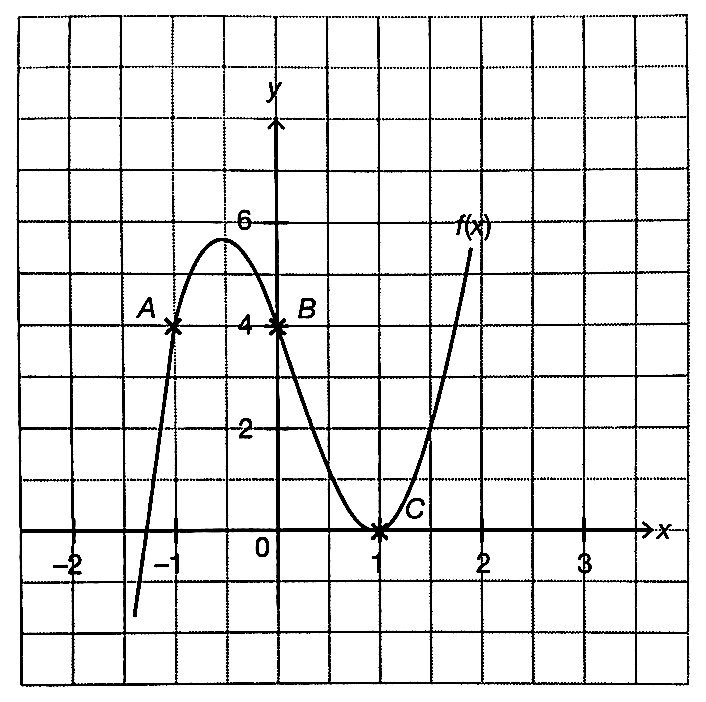
\includegraphics[width=0.3\textwidth]{./images/q24.jpeg}
              \end{center}
              \begin{enumerate}
                  \item Find the gradient function of the tangent to the curve $f(x)$.
                  \item \begin{enumerate}
                            \item Find the values of gradient of the tangents to the curve at points $A$, $B$,
                                  and $C$.
                            \item Hence, elaborate the situations of the tangents at points $A$, $B$, and $C$
                                  based on the values of the gradient obtained in (i).
                        \end{enumerate}
              \end{enumerate}
        \item Find the gradient of the tangent for each of the following furves at the given
              point $P$.
              \begin{enumerate}
                  \item $y = 4x - \dfrac{8}{x}; P(4, 14)$
                  \item $y = \dfrac{4 - 3x^2}{3-2x}; P(2, 8)$
              \end{enumerate}
        \item \begin{enumerate}
                  \item Find the value of gradient of the tangent to the curve $y = 2x^3 - 3x^2$ when
                        $x = 1$.
                  \item Find the coordinates of points to the curve $y = \dfrac{x^3}{3} + x^2 - 1$ such
                        that the gradient to the curve at the points is $8$.
                  \item Given the curve $y = ax^2 + bx + 3$ has the gradient $5$ when $x = 2$ and the
                        gradient $0$ when $x = -3$. Determine the values of $a$ and $b$.
              \end{enumerate}
        \item Find the equations of tangent and normal to the curve $y = 8 - 2x - x^2$ at
              each of the following points.
              \begin{enumerate}
                  \item $A(1, 5)$
                  \item $C(-1, 9)$
              \end{enumerate}
        \item \begin{enumerate}
                  \item Find the equation of normal to the curve $y = 3x^2 + 8x - 7$ at point $(-2,
                            6)$.
                  \item Given the tangent to the curve $y = ax^2 + bx$ at the point $P(4, 8)$ is
                        perpendicular to the straight line that passes through the point $A(4, 1)$ and
                        the point $B(12, 0)$. Find the values of $a$ and $b$.
              \end{enumerate}
        \item Find the coordinates of the turning points for each of the following curves.
              \begin{enumerate}
                  \item $y = 5x^2 - 2x + 1$
                  \item $y = \dfrac{x^2}{x+1}$
                  \item $y = 7 - x^3$
                        Hence, determine the nature of each point with
                        \begin{enumerate}
                            \item the tangent sketching method.
                            \item the second order derivative method.
                        \end{enumerate}
              \end{enumerate}
        \item Solve the following problems related to stationary points.
              \begin{enumerate}
                  \item The following diagram shows the plan of a cuboid in which its centre in the
                        shape of a cylinder is taken out. The cuboid measures $3x\textit{cm} \times
                            2x\textit{cm} \times (45 - 5x)\textit{cm}$.
                        \begin{center}
                            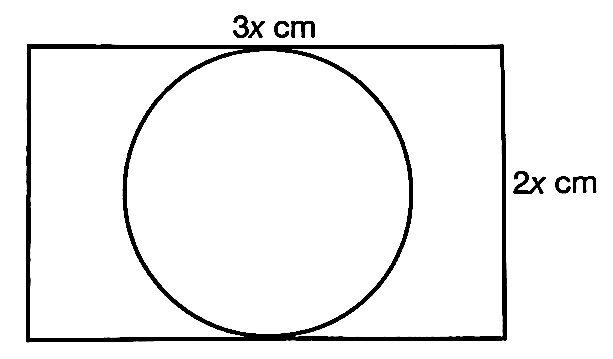
\includegraphics[width=0.3\textwidth]{./images/q30.jpeg}
                        \end{center}
                        Find the value of $x$ that makes the volume of the cylinder taken out a maximum.
                  \item Given $A = bh$ where $b^2 + h^2 = 40$ and $b, h > 0$. Find the values of $b$
                        and $h$ so that $A$ becomes a stationary point and show that the value of $A$
                        is maximum.
                  \item A piece of wire with a length of $120\textit{cm}$ is divided into two parts
                        where is each is bent to form an equilateral triangle with an edge of
                        $x\textit{cm}$ and a square with an edge of $y\textit{cm}$ respectively express
                        $y$ in terms of $x$. Hencex show that the total area of both shapes,
                        $A\textit{cm}^2$ is given by
                        \[A = \dfrac{9{(40 - x)}^2 + 4\sqrt{3}x^2}{16}\]
                        Calculate the value of $x$ so that $A$ has a stationary value. Determine
                        whether this value of $x$ makes $A$ a maximum of a minimum.
              \end{enumerate}
        \item Chan wants to build two separate pens by using a fenc of $100\textit{m}$. Both
              pens are square in shape.
              \begin{center}
                  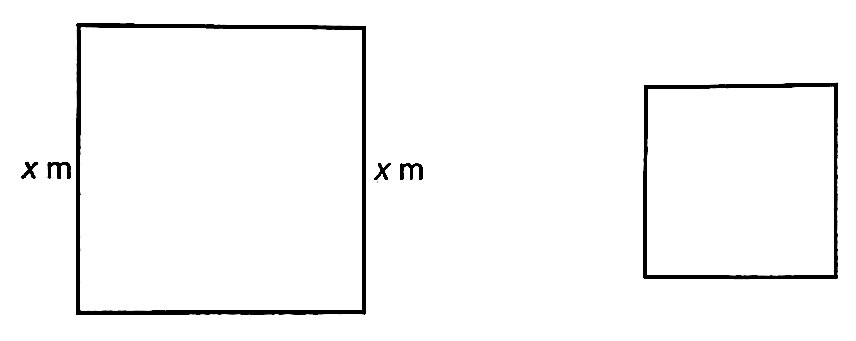
\includegraphics[width=0.4\textwidth]{./images/q30_2.jpeg}
              \end{center}
              If the edge of the larger pen is $x\textit{m}$,
              \begin{enumerate}
                  \item find the length of the side of the smaller pen in terms of $x$.
                  \item find the value of $x$ such that the total area of both pens is minimum.
              \end{enumerate}
        \item Solve the following problems related to the rates of change.
              \begin{enumerate}
                  \item The total surface area, $A\textit{cm}^2$, of a metal solid which consists of a
                        cone and a cylinder with a common radius, $r\textit{cm}$ is given by $A =
                            2\pi\left(\dfrac{18}{r} + \dfrac{r^2}{3}\right)$. When it is heated, its total
                        surface area changes at the rate of $2.1\pi \textit{cm}^2s^{-1}$. Find the rate
                        of change of the radius, in $\textit{cm} s^{-1}$, at the instant $r =
                            6\textit{cm}$.
                  \item A spherical balloon experiences a constant rate of increase of
                        $6\textit{cm}^2s^{-1}$.
                        \begin{center}
                            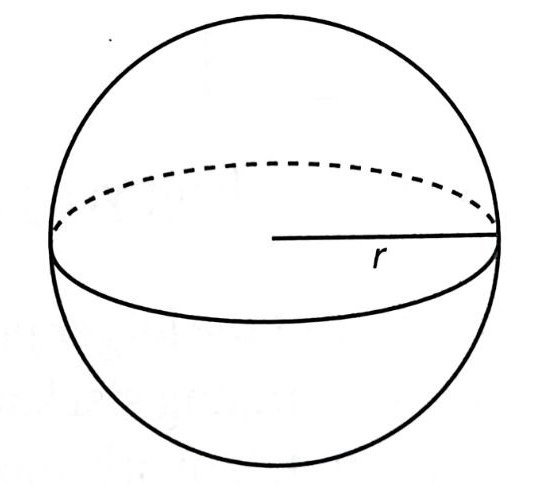
\includegraphics[width=0.3\textwidth]{./images/q31.jpeg}
                        \end{center}
                        At the instant when the radius is 5cm, find
                        \begin{enumerate}
                            \item the rate of increase, in $cm s^{-1}$, of the radius.
                            \item the rate of increase if volume, in $cm^3 s^{-1}$, of the sphere.
                        \end{enumerate}
                  \item The following diagram shows a container in the shape of a cone. Given its
                        height is equal to its base radius. Water is poured into the container at the
                        rate of $80\textit{cm}^3s^{-1}$. The volume of the water in the container is
                        $\dfrac{1}{3}\pi x^3\textit{cm}^3$, when the depth of the water is
                        $x\textit{cm}$.
                        \begin{center}
                            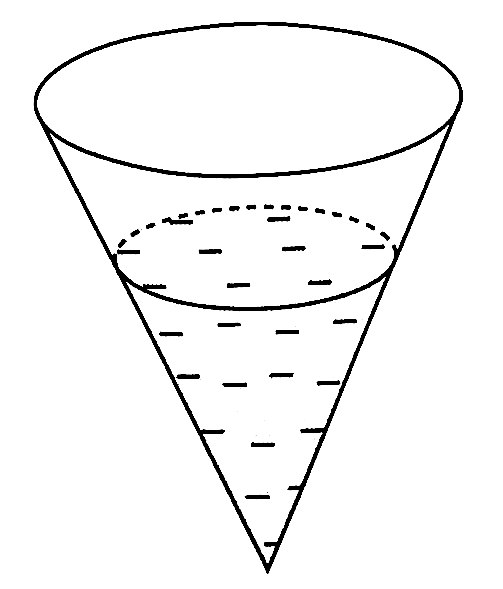
\includegraphics[width=0.2\textwidth]{./images/q31_2.jpeg}
                        \end{center}
                        Calculate, at the instant when the depth of the water is $10\textit{cm}$,
                        \begin{enumerate}
                            \item the rate of increase of the depth, in $\textit{cm} s^{-1}$, of the water.
                            \item the rate of increase of the horizontal surface area, in $\textit{cm}^2 s^{-1}$,
                                  of the water.
                        \end{enumerate}
              \end{enumerate}

        \item Solve the following problems related to the small changes and aproximations.
              \begin{enumerate}
                  \item Given that $y = 2x^3 - 5x^2 + x - 1$, find the value of $\dfrac{dy}{dx}$ when
                        $x = 1$. Hence, find the small changes in $y$ when $x$ increases from $1$ to
                        $1.02$.
                  \item Given the equation of a curve is $y = \dfrac{9}{{(2x - 5)}^2}$, find, in terms
                        of $p$, where $p$ is a small value, the approximate change in
                        \begin{enumerate}
                            \item $y$ when $x$ increases from $3$ to $3 + p$.
                            \item $x$ when $y$ decreases from $1$ to $1 - p$.
                        \end{enumerate}
                  \item Given $y = x^4$, by using the calculus method, find the approximate value of
                        \begin{enumerate}
                            \item $2.03^4$.
                            \item $1.99^4$.
                        \end{enumerate}
              \end{enumerate}
        \item A hemispherical bowl of radius $R\textit{cm}$ is filled with water to a depth
              of $h\textit{cm}$.
              \begin{center}
                  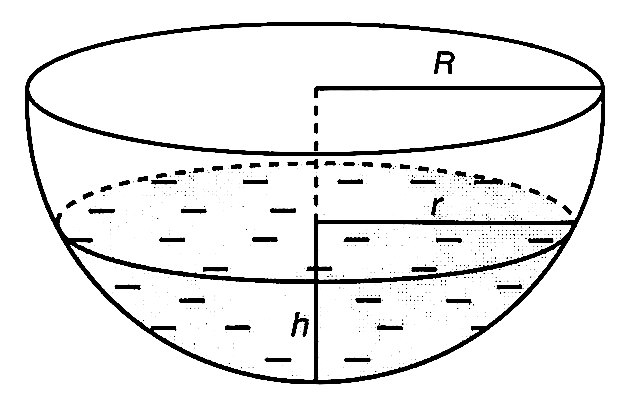
\includegraphics[width=0.3\textwidth]{./images/q33.jpeg}
              \end{center}
              The volume of the water in the bowl is given by $V = \dfrac{\pi}{3}(3Rh^2 - h^3)$.
              \begin{enumerate}
                  \item Show that the radius of the water surface, $r$, is given by $r = \sqrt{2Rh -
                                h^2}$.
                  \item Water is poured into the bown at a constand rate of $300cm^3s^{-1}$. Find, in
                        terms of $R$, the rate of increase of the surface area, in $cm^2
                            \textit{min}^{-1}$, of the water when $2h = R$.
              \end{enumerate}
    \end{enumerate}
\end{multicols*}

\end{document}